\documentclass[1p]{elsarticle_modified}
%\bibliographystyle{elsarticle-num}

%\usepackage[colorlinks]{hyperref}
%\usepackage{abbrmath_seonhwa} %\Abb, \Ascr, \Acal ,\Abf, \Afrak
\usepackage{amsfonts}
\usepackage{amssymb}
\usepackage{amsmath}
\usepackage{amsthm}
\usepackage{scalefnt}
\usepackage{amsbsy}
\usepackage{kotex}
\usepackage{caption}
\usepackage{subfig}
\usepackage{color}
\usepackage{graphicx}
\usepackage{xcolor} %% white, black, red, green, blue, cyan, magenta, yellow
\usepackage{float}
\usepackage{setspace}
\usepackage{hyperref}

\usepackage{tikz}
\usetikzlibrary{arrows}

\usepackage{multirow}
\usepackage{array} % fixed length table
\usepackage{hhline}

%%%%%%%%%%%%%%%%%%%%%
\makeatletter
\renewcommand*\env@matrix[1][\arraystretch]{%
	\edef\arraystretch{#1}%
	\hskip -\arraycolsep
	\let\@ifnextchar\new@ifnextchar
	\array{*\c@MaxMatrixCols c}}
\makeatother %https://tex.stackexchange.com/questions/14071/how-can-i-increase-the-line-spacing-in-a-matrix
%%%%%%%%%%%%%%%

\usepackage[normalem]{ulem}

\newcommand{\msout}[1]{\ifmmode\text{\sout{\ensuremath{#1}}}\else\sout{#1}\fi}
%SOURCE: \msout is \stkout macro in https://tex.stackexchange.com/questions/20609/strikeout-in-math-mode

\newcommand{\cancel}[1]{
	\ifmmode
	{\color{red}\msout{#1}}
	\else
	{\color{red}\sout{#1}}
	\fi
}

\newcommand{\add}[1]{
	{\color{blue}\uwave{#1}}
}

\newcommand{\replace}[2]{
	\ifmmode
	{\color{red}\msout{#1}}{\color{blue}\uwave{#2}}
	\else
	{\color{red}\sout{#1}}{\color{blue}\uwave{#2}}
	\fi
}

\newcommand{\Sol}{\mathcal{S}} %segment
\newcommand{\D}{D} %diagram
\newcommand{\A}{\mathcal{A}} %arc


%%%%%%%%%%%%%%%%%%%%%%%%%%%%%5 test

\def\sl{\operatorname{\textup{SL}}(2,\Cbb)}
\def\psl{\operatorname{\textup{PSL}}(2,\Cbb)}
\def\quan{\mkern 1mu \triangleright \mkern 1mu}

\theoremstyle{definition}
\newtheorem{thm}{Theorem}[section]
\newtheorem{prop}[thm]{Proposition}
\newtheorem{lem}[thm]{Lemma}
\newtheorem{ques}[thm]{Question}
\newtheorem{cor}[thm]{Corollary}
\newtheorem{defn}[thm]{Definition}
\newtheorem{exam}[thm]{Example}
\newtheorem{rmk}[thm]{Remark}
\newtheorem{alg}[thm]{Algorithm}

\newcommand{\I}{\sqrt{-1}}
\begin{document}

%\begin{frontmatter}
%
%\title{Boundary parabolic representations of knots up to 8 crossings}
%
%%% Group authors per affiliation:
%\author{Yunhi Cho} 
%\address{Department of Mathematics, University of Seoul, Seoul, Korea}
%\ead{yhcho@uos.ac.kr}
%
%
%\author{Seonhwa Kim} %\fnref{s_kim}}
%\address{Center for Geometry and Physics, Institute for Basic Science, Pohang, 37673, Korea}
%\ead{ryeona17@ibs.re.kr}
%
%\author{Hyuk Kim}
%\address{Department of Mathematical Sciences, Seoul National University, Seoul 08826, Korea}
%\ead{hyukkim@snu.ac.kr}
%
%\author{Seokbeom Yoon}
%\address{Department of Mathematical Sciences, Seoul National University, Seoul, 08826,  Korea}
%\ead{sbyoon15@snu.ac.kr}
%
%\begin{abstract}
%We find all boundary parabolic representation of knots up to 8 crossings.
%
%\end{abstract}
%\begin{keyword}
%    \MSC[2010] 57M25 
%\end{keyword}
%
%\end{frontmatter}

%\linenumbers
%\tableofcontents
%
\newcommand\colored[1]{\textcolor{white}{\rule[-0.35ex]{0.8em}{1.4ex}}\kern-0.8em\color{red} #1}%
%\newcommand\colored[1]{\textcolor{white}{ #1}\kern-2.17ex	\textcolor{white}{ #1}\kern-1.81ex	\textcolor{white}{ #1}\kern-2.15ex\color{red}#1	}

{\Large $\underline{12n_{0343}~(K12n_{0343})}$}

\setlength{\tabcolsep}{10pt}
\renewcommand{\arraystretch}{1.6}
\vspace{1cm}\begin{tabular}{m{100pt}>{\centering\arraybackslash}m{274pt}}
\multirow{5}{120pt}{
	\centering
	\includegraphics[width=112pt]{../../../GIT/diagram.site/Diagrams/png/2432_12n_0343.png}\\
\ \ \ A knot diagram\footnotemark}&
\allowdisplaybreaks
\textbf{Linearized knot diagam} \\
\cline{2-2}
 &
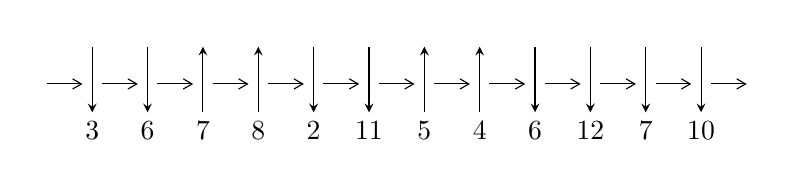
\begin{tikzpicture}[x=20pt, y=17pt]
	% nodes
	\node (C0) at (0, 0) {};
	\node (C1) at (1, 0) {};
	\node (C1U) at (1, +1) {};
	\node (C1D) at (1, -1) {3};

	\node (C2) at (2, 0) {};
	\node (C2U) at (2, +1) {};
	\node (C2D) at (2, -1) {6};

	\node (C3) at (3, 0) {};
	\node (C3U) at (3, +1) {};
	\node (C3D) at (3, -1) {7};

	\node (C4) at (4, 0) {};
	\node (C4U) at (4, +1) {};
	\node (C4D) at (4, -1) {8};

	\node (C5) at (5, 0) {};
	\node (C5U) at (5, +1) {};
	\node (C5D) at (5, -1) {2};

	\node (C6) at (6, 0) {};
	\node (C6U) at (6, +1) {};
	\node (C6D) at (6, -1) {11};

	\node (C7) at (7, 0) {};
	\node (C7U) at (7, +1) {};
	\node (C7D) at (7, -1) {5};

	\node (C8) at (8, 0) {};
	\node (C8U) at (8, +1) {};
	\node (C8D) at (8, -1) {4};

	\node (C9) at (9, 0) {};
	\node (C9U) at (9, +1) {};
	\node (C9D) at (9, -1) {6};

	\node (C10) at (10, 0) {};
	\node (C10U) at (10, +1) {};
	\node (C10D) at (10, -1) {12};

	\node (C11) at (11, 0) {};
	\node (C11U) at (11, +1) {};
	\node (C11D) at (11, -1) {7};

	\node (C12) at (12, 0) {};
	\node (C12U) at (12, +1) {};
	\node (C12D) at (12, -1) {10};
	\node (C13) at (13, 0) {};

	% arrows
	\draw[->,>={angle 60}]
	(C0) edge (C1) (C1) edge (C2) (C2) edge (C3) (C3) edge (C4) (C4) edge (C5) (C5) edge (C6) (C6) edge (C7) (C7) edge (C8) (C8) edge (C9) (C9) edge (C10) (C10) edge (C11) (C11) edge (C12) (C12) edge (C13) ;	\draw[->,>=stealth]
	(C1U) edge (C1D) (C2U) edge (C2D) (C3D) edge (C3U) (C4D) edge (C4U) (C5U) edge (C5D) (C6U) edge (C6D) (C7D) edge (C7U) (C8D) edge (C8U) (C9U) edge (C9D) (C10U) edge (C10D) (C11U) edge (C11D) (C12U) edge (C12D) ;
	\end{tikzpicture} \\
\hhline{~~} \\& 
\textbf{Solving Sequence} \\ \cline{2-2} 
 &
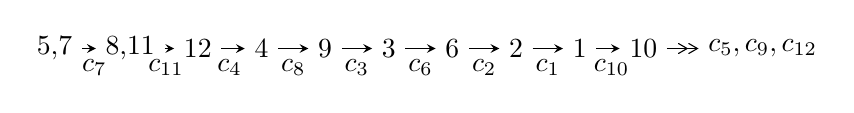
\begin{tikzpicture}[x=23pt, y=7pt]
	% node
	\node (A0) at (-1/8, 0) {5,7};
	\node (A1) at (17/16, 0) {8,11};
	\node (A2) at (17/8, 0) {12};
	\node (A3) at (25/8, 0) {4};
	\node (A4) at (33/8, 0) {9};
	\node (A5) at (41/8, 0) {3};
	\node (A6) at (49/8, 0) {6};
	\node (A7) at (57/8, 0) {2};
	\node (A8) at (65/8, 0) {1};
	\node (A9) at (73/8, 0) {10};
	\node (C1) at (1/2, -1) {$c_{7}$};
	\node (C2) at (13/8, -1) {$c_{11}$};
	\node (C3) at (21/8, -1) {$c_{4}$};
	\node (C4) at (29/8, -1) {$c_{8}$};
	\node (C5) at (37/8, -1) {$c_{3}$};
	\node (C6) at (45/8, -1) {$c_{6}$};
	\node (C7) at (53/8, -1) {$c_{2}$};
	\node (C8) at (61/8, -1) {$c_{1}$};
	\node (C9) at (69/8, -1) {$c_{10}$};
	\node (A10) at (11, 0) {$c_{5},c_{9},c_{12}$};

	% edge
	\draw[->,>=stealth]	
	(A0) edge (A1) (A1) edge (A2) (A2) edge (A3) (A3) edge (A4) (A4) edge (A5) (A5) edge (A6) (A6) edge (A7) (A7) edge (A8) (A8) edge (A9) ;
	\draw[->>,>={angle 60}]	
	(A9) edge (A10);
\end{tikzpicture} \\ 

\end{tabular} \\

\footnotetext{
The image of knot diagram is generated by the software ``\textbf{Draw programme}" developed by Andrew Bartholomew(\url{http://www.layer8.co.uk/maths/draw/index.htm\#Running-draw}), where we modified some parts for our purpose(\url{https://github.com/CATsTAILs/LinksPainter}).
}\phantom \\ \newline 
\centering \textbf{Ideals for irreducible components\footnotemark of $X_{\text{par}}$} 
 
\begin{align*}
I^u_{1}&=\langle 
2.35414\times10^{25} u^{37}+6.36686\times10^{22} u^{36}+\cdots+1.08506\times10^{26} b+7.17457\times10^{26},\\
\phantom{I^u_{1}}&\phantom{= \langle  }-6.03496\times10^{25} u^{37}-5.08818\times10^{25} u^{36}+\cdots+1.08506\times10^{26} a-2.36548\times10^{27},\;u^{38}+u^{37}+\cdots+48 u+8\rangle \\
I^u_{2}&=\langle 
4 a^2 u+2 a^2+9 b-9,\;4 a^3+4 a u-2 a-5 u-2,\;u^2+2\rangle \\
\\
I^v_{1}&=\langle 
a,\;b+v+1,\;v^3+2 v^2+v+1\rangle \\
\end{align*}
\raggedright * 3 irreducible components of $\dim_{\mathbb{C}}=0$, with total 47 representations.\\
\footnotetext{All coefficients of polynomials are rational numbers. But the coefficients are sometimes approximated in decimal forms when there is not enough margin.}
\newpage
\renewcommand{\arraystretch}{1}
\centering \section*{I. $I^u_{1}= \langle 2.35\times10^{25} u^{37}+6.37\times10^{22} u^{36}+\cdots+1.09\times10^{26} b+7.17\times10^{26},\;-6.03\times10^{25} u^{37}-5.09\times10^{25} u^{36}+\cdots+1.09\times10^{26} a-2.37\times10^{27},\;u^{38}+u^{37}+\cdots+48 u+8 \rangle$}
\flushleft \textbf{(i) Arc colorings}\\
\begin{tabular}{m{7pt} m{180pt} m{7pt} m{180pt} }
\flushright $a_{5}=$&$\begin{pmatrix}0\\u\end{pmatrix}$ \\
\flushright $a_{7}=$&$\begin{pmatrix}1\\0\end{pmatrix}$ \\
\flushright $a_{8}=$&$\begin{pmatrix}1\\- u^2\end{pmatrix}$ \\
\flushright $a_{11}=$&$\begin{pmatrix}0.556188 u^{37}+0.468931 u^{36}+\cdots+66.0065 u+21.8004\\-0.216959 u^{37}-0.000586775 u^{36}+\cdots-20.1029 u-6.61215\end{pmatrix}$ \\
\flushright $a_{12}=$&$\begin{pmatrix}0.773147 u^{37}+0.469518 u^{36}+\cdots+86.1094 u+28.4126\\-0.216959 u^{37}-0.000586775 u^{36}+\cdots-20.1029 u-6.61215\end{pmatrix}$ \\
\flushright $a_{4}=$&$\begin{pmatrix}- u\\u^3+u\end{pmatrix}$ \\
\flushright $a_{9}=$&$\begin{pmatrix}u^2+1\\- u^4-2 u^2\end{pmatrix}$ \\
\flushright $a_{3}=$&$\begin{pmatrix}- u^3-2 u\\u^3+u\end{pmatrix}$ \\
\flushright $a_{6}=$&$\begin{pmatrix}0.540457 u^{37}+0.513997 u^{36}+\cdots+61.5142 u+18.9792\\0.118184 u^{37}-0.103841 u^{36}+\cdots-10.8806 u-1.99927\end{pmatrix}$ \\
\flushright $a_{2}=$&$\begin{pmatrix}-0.931000 u^{37}-0.423758 u^{36}+\cdots-46.4113 u-16.9685\\0.272358 u^{37}+0.0136024 u^{36}+\cdots-4.22233 u-0.0113747\end{pmatrix}$ \\
\flushright $a_{1}=$&$\begin{pmatrix}-1.34851 u^{37}-0.494264 u^{36}+\cdots-50.4295 u-19.4015\\0.448295 u^{37}+0.0937407 u^{36}+\cdots+2.84945 u+2.20997\end{pmatrix}$ \\
\flushright $a_{10}=$&$\begin{pmatrix}-0.237267 u^{37}-0.770027 u^{36}+\cdots-6.76734 u+5.06203\\0.216015 u^{37}+0.558969 u^{36}+\cdots+14.6047 u+0.926935\end{pmatrix}$\\&\end{tabular}
\flushleft \textbf{(ii) Obstruction class $= -1$}\\~\\
\flushleft \textbf{(iii) Cusp Shapes $= \frac{213942583101129059255880827}{108505904310727076649467996} u^{37}+\frac{149904830321107825585617651}{108505904310727076649467996} u^{36}+\cdots+\frac{5023310390844651983501342066}{27126476077681769162366999} u+\frac{1400899338503733927958392044}{27126476077681769162366999}$}\\~\\
\newpage\renewcommand{\arraystretch}{1}
\flushleft \textbf{(iv) u-Polynomials at the component}\newline \\
\begin{tabular}{m{50pt}|m{274pt}}
Crossings & \hspace{64pt}u-Polynomials at each crossing \\
\hline $$\begin{aligned}c_{1}\end{aligned}$$&$\begin{aligned}
&u^{38}+10 u^{37}+\cdots-24 u+1
\end{aligned}$\\
\hline $$\begin{aligned}c_{2},c_{5}\end{aligned}$$&$\begin{aligned}
&u^{38}+4 u^{37}+\cdots+4 u-1
\end{aligned}$\\
\hline $$\begin{aligned}c_{3}\end{aligned}$$&$\begin{aligned}
&u^{38}- u^{37}+\cdots-16 u+8
\end{aligned}$\\
\hline $$\begin{aligned}c_{4},c_{7},c_{8}\end{aligned}$$&$\begin{aligned}
&u^{38}+u^{37}+\cdots+48 u+8
\end{aligned}$\\
\hline $$\begin{aligned}c_{6},c_{11}\end{aligned}$$&$\begin{aligned}
&u^{38}-2 u^{37}+\cdots+u-3
\end{aligned}$\\
\hline $$\begin{aligned}c_{9}\end{aligned}$$&$\begin{aligned}
&u^{38}+2 u^{37}+\cdots-3029 u-7419
\end{aligned}$\\
\hline $$\begin{aligned}c_{10},c_{12}\end{aligned}$$&$\begin{aligned}
&u^{38}+8 u^{37}+\cdots+85 u+9
\end{aligned}$\\
\hline
\end{tabular}\\~\\
\newpage\renewcommand{\arraystretch}{1}
\flushleft \textbf{(v) Riley Polynomials at the component}\newline \\
\begin{tabular}{m{50pt}|m{274pt}}
Crossings & \hspace{64pt}Riley Polynomials at each crossing \\
\hline $$\begin{aligned}c_{1}\end{aligned}$$&$\begin{aligned}
&y^{38}+46 y^{37}+\cdots+1128 y+1
\end{aligned}$\\
\hline $$\begin{aligned}c_{2},c_{5}\end{aligned}$$&$\begin{aligned}
&y^{38}-10 y^{37}+\cdots+24 y+1
\end{aligned}$\\
\hline $$\begin{aligned}c_{3}\end{aligned}$$&$\begin{aligned}
&y^{38}-53 y^{37}+\cdots+896 y+64
\end{aligned}$\\
\hline $$\begin{aligned}c_{4},c_{7},c_{8}\end{aligned}$$&$\begin{aligned}
&y^{38}+31 y^{37}+\cdots-512 y+64
\end{aligned}$\\
\hline $$\begin{aligned}c_{6},c_{11}\end{aligned}$$&$\begin{aligned}
&y^{38}-8 y^{37}+\cdots-85 y+9
\end{aligned}$\\
\hline $$\begin{aligned}c_{9}\end{aligned}$$&$\begin{aligned}
&y^{38}+120 y^{37}+\cdots-2146915177 y+55041561
\end{aligned}$\\
\hline $$\begin{aligned}c_{10},c_{12}\end{aligned}$$&$\begin{aligned}
&y^{38}+48 y^{37}+\cdots+1091 y+81
\end{aligned}$\\
\hline
\end{tabular}\\~\\
\newpage\flushleft \textbf{(vi) Complex Volumes and Cusp Shapes}
$$\begin{array}{c|c|c}  
\text{Solutions to }I^u_{1}& \I (\text{vol} + \sqrt{-1}CS) & \text{Cusp shape}\\
 \hline 
\begin{aligned}
u &= -1.053800 + 0.148639 I \\
a &= -0.35198 - 1.75546 I \\
b &= \phantom{-}0.976993 + 0.905951 I\end{aligned}
 & \phantom{-}12.2690 - 7.2289 I & -0.96626 + 4.68407 I \\ \hline\begin{aligned}
u &= -1.053800 - 0.148639 I \\
a &= -0.35198 + 1.75546 I \\
b &= \phantom{-}0.976993 - 0.905951 I\end{aligned}
 & \phantom{-}12.2690 + 7.2289 I & -0.96626 - 4.68407 I \\ \hline\begin{aligned}
u &= -0.057390 + 0.931497 I \\
a &= \phantom{-}0.49812 + 1.63735 I \\
b &= -0.893541 - 0.823917 I\end{aligned}
 & \phantom{-}0.10554 - 3.06762 I & -6.46786 + 2.97828 I \\ \hline\begin{aligned}
u &= -0.057390 - 0.931497 I \\
a &= \phantom{-}0.49812 - 1.63735 I \\
b &= -0.893541 + 0.823917 I\end{aligned}
 & \phantom{-}0.10554 + 3.06762 I & -6.46786 - 2.97828 I \\ \hline\begin{aligned}
u &= \phantom{-}1.064480 + 0.094759 I \\
a &= -0.73343 - 1.41153 I \\
b &= \phantom{-}0.912968 + 0.941319 I\end{aligned}
 & \phantom{-}12.47990 + 0.43824 I & -0.562427 - 0.044649 I \\ \hline\begin{aligned}
u &= \phantom{-}1.064480 - 0.094759 I \\
a &= -0.73343 + 1.41153 I \\
b &= \phantom{-}0.912968 - 0.941319 I\end{aligned}
 & \phantom{-}12.47990 - 0.43824 I & -0.562427 + 0.044649 I \\ \hline\begin{aligned}
u &= \phantom{-}0.156341 + 1.111710 I \\
a &= \phantom{-}1.23758 + 0.87855 I \\
b &= \phantom{-}0.929752 - 0.586434 I\end{aligned}
 & -1.21085 + 3.08073 I & -5.55249 - 3.17627 I \\ \hline\begin{aligned}
u &= \phantom{-}0.156341 - 1.111710 I \\
a &= \phantom{-}1.23758 - 0.87855 I \\
b &= \phantom{-}0.929752 + 0.586434 I\end{aligned}
 & -1.21085 - 3.08073 I & -5.55249 + 3.17627 I \\ \hline\begin{aligned}
u &= -0.191591 + 1.141470 I \\
a &= -1.71195 + 0.26865 I \\
b &= -1.018780 + 0.030482 I\end{aligned}
 & -4.76428 - 2.22122 I & -10.55897 + 3.42071 I \\ \hline\begin{aligned}
u &= -0.191591 - 1.141470 I \\
a &= -1.71195 - 0.26865 I \\
b &= -1.018780 - 0.030482 I\end{aligned}
 & -4.76428 + 2.22122 I & -10.55897 - 3.42071 I\\
 \hline 
 \end{array}$$\newpage$$\begin{array}{c|c|c}  
\text{Solutions to }I^u_{1}& \I (\text{vol} + \sqrt{-1}CS) & \text{Cusp shape}\\
 \hline 
\begin{aligned}
u &= -0.271471 + 0.749945 I \\
a &= -0.032046 - 0.267481 I \\
b &= \phantom{-}0.626757 - 0.614277 I\end{aligned}
 & -0.20728 + 1.53818 I & -4.56900 - 2.28483 I \\ \hline\begin{aligned}
u &= -0.271471 - 0.749945 I \\
a &= -0.032046 + 0.267481 I \\
b &= \phantom{-}0.626757 + 0.614277 I\end{aligned}
 & -0.20728 - 1.53818 I & -4.56900 + 2.28483 I \\ \hline\begin{aligned}
u &= \phantom{-}0.418841 + 1.156790 I \\
a &= -0.417466 - 0.176902 I \\
b &= \phantom{-}0.386654 + 0.764550 I\end{aligned}
 & \phantom{-}0.11970 + 3.73317 I & -2.97329 - 3.30525 I \\ \hline\begin{aligned}
u &= \phantom{-}0.418841 - 1.156790 I \\
a &= -0.417466 + 0.176902 I \\
b &= \phantom{-}0.386654 - 0.764550 I\end{aligned}
 & \phantom{-}0.11970 - 3.73317 I & -2.97329 + 3.30525 I \\ \hline\begin{aligned}
u &= \phantom{-}0.714927 + 0.180259 I \\
a &= \phantom{-}0.324913 - 1.250580 I \\
b &= -0.617135 + 0.730511 I\end{aligned}
 & \phantom{-}3.04719 + 0.49757 I & \phantom{-}1.21153 - 1.20838 I \\ \hline\begin{aligned}
u &= \phantom{-}0.714927 - 0.180259 I \\
a &= \phantom{-}0.324913 + 1.250580 I \\
b &= -0.617135 - 0.730511 I\end{aligned}
 & \phantom{-}3.04719 - 0.49757 I & \phantom{-}1.21153 + 1.20838 I \\ \hline\begin{aligned}
u &= \phantom{-}0.227184 + 0.682533 I \\
a &= \phantom{-}0.429035 + 0.360906 I \\
b &= \phantom{-}0.320049 - 0.507052 I\end{aligned}
 & -0.238421 + 1.266880 I & -2.42303 - 5.08329 I \\ \hline\begin{aligned}
u &= \phantom{-}0.227184 - 0.682533 I \\
a &= \phantom{-}0.429035 - 0.360906 I \\
b &= \phantom{-}0.320049 + 0.507052 I\end{aligned}
 & -0.238421 - 1.266880 I & -2.42303 + 5.08329 I \\ \hline\begin{aligned}
u &= -0.092432 + 1.311290 I \\
a &= \phantom{-}0.14750 - 1.68723 I \\
b &= \phantom{-}0.688190 + 0.376073 I\end{aligned}
 & -6.50773 - 1.47983 I & -9.20328 + 4.48160 I \\ \hline\begin{aligned}
u &= -0.092432 - 1.311290 I \\
a &= \phantom{-}0.14750 + 1.68723 I \\
b &= \phantom{-}0.688190 - 0.376073 I\end{aligned}
 & -6.50773 + 1.47983 I & -9.20328 - 4.48160 I\\
 \hline 
 \end{array}$$\newpage$$\begin{array}{c|c|c}  
\text{Solutions to }I^u_{1}& \I (\text{vol} + \sqrt{-1}CS) & \text{Cusp shape}\\
 \hline 
\begin{aligned}
u &= -0.366037 + 1.277380 I \\
a &= \phantom{-}1.32644 - 1.19862 I \\
b &= \phantom{-}1.025390 + 0.488331 I\end{aligned}
 & -1.99066 - 8.34590 I & -7.38920 + 8.20539 I \\ \hline\begin{aligned}
u &= -0.366037 - 1.277380 I \\
a &= \phantom{-}1.32644 + 1.19862 I \\
b &= \phantom{-}1.025390 - 0.488331 I\end{aligned}
 & -1.99066 + 8.34590 I & -7.38920 - 8.20539 I \\ \hline\begin{aligned}
u &= -0.669684 + 0.020164 I \\
a &= -0.022217 + 1.347390 I \\
b &= -0.937251 - 0.595896 I\end{aligned}
 & \phantom{-}1.98177 - 4.45651 I & -1.06472 + 6.47147 I \\ \hline\begin{aligned}
u &= -0.669684 - 0.020164 I \\
a &= -0.022217 - 1.347390 I \\
b &= -0.937251 + 0.595896 I\end{aligned}
 & \phantom{-}1.98177 + 4.45651 I & -1.06472 - 6.47147 I \\ \hline\begin{aligned}
u &= -0.618417 + 1.229390 I \\
a &= \phantom{-}0.511319 - 0.554883 I \\
b &= -0.923330 + 0.927636 I\end{aligned}
 & \phantom{-}8.97672 + 1.36657 I & -4.00000 + 0. I\phantom{ +0.000000I} \\ \hline\begin{aligned}
u &= -0.618417 - 1.229390 I \\
a &= \phantom{-}0.511319 + 0.554883 I \\
b &= -0.923330 - 0.927636 I\end{aligned}
 & \phantom{-}8.97672 - 1.36657 I & -4.00000 + 0. I\phantom{ +0.000000I} \\ \hline\begin{aligned}
u &= \phantom{-}0.590971 + 1.277150 I \\
a &= -0.48725 - 1.50500 I \\
b &= -0.961686 + 0.907689 I\end{aligned}
 & \phantom{-}8.85183 + 5.38651 I & \phantom{-0.000000 } 0 \\ \hline\begin{aligned}
u &= \phantom{-}0.590971 - 1.277150 I \\
a &= -0.48725 + 1.50500 I \\
b &= -0.961686 - 0.907689 I\end{aligned}
 & \phantom{-}8.85183 - 5.38651 I & \phantom{-0.000000 } 0 \\ \hline\begin{aligned}
u &= \phantom{-}0.02483 + 1.43079 I \\
a &= \phantom{-}0.637356 + 0.570357 I \\
b &= \phantom{-}0.863543 - 0.756976 I\end{aligned}
 & -1.89195 + 2.85204 I & -4.00000 + 0. I\phantom{ +0.000000I} \\ \hline\begin{aligned}
u &= \phantom{-}0.02483 - 1.43079 I \\
a &= \phantom{-}0.637356 - 0.570357 I \\
b &= \phantom{-}0.863543 + 0.756976 I\end{aligned}
 & -1.89195 - 2.85204 I & -4.00000 + 0. I\phantom{ +0.000000I}\\
 \hline 
 \end{array}$$\newpage$$\begin{array}{c|c|c}  
\text{Solutions to }I^u_{1}& \I (\text{vol} + \sqrt{-1}CS) & \text{Cusp shape}\\
 \hline 
\begin{aligned}
u &= -0.03651 + 1.47301 I \\
a &= -1.199870 + 0.246838 I \\
b &= -0.661912 + 0.244654 I\end{aligned}
 & -7.07448 + 0.98863 I & \phantom{-0.000000 } 0 \\ \hline\begin{aligned}
u &= -0.03651 - 1.47301 I \\
a &= -1.199870 - 0.246838 I \\
b &= -0.661912 - 0.244654 I\end{aligned}
 & -7.07448 - 0.98863 I & \phantom{-0.000000 } 0 \\ \hline\begin{aligned}
u &= \phantom{-}0.50808 + 1.40664 I \\
a &= \phantom{-}0.592702 + 0.296009 I \\
b &= -0.857340 - 0.944975 I\end{aligned}
 & \phantom{-}7.77909 + 6.04150 I & \phantom{-0.000000 } 0 \\ \hline\begin{aligned}
u &= \phantom{-}0.50808 - 1.40664 I \\
a &= \phantom{-}0.592702 - 0.296009 I \\
b &= -0.857340 + 0.944975 I\end{aligned}
 & \phantom{-}7.77909 - 6.04150 I & \phantom{-0.000000 } 0 \\ \hline\begin{aligned}
u &= -0.48076 + 1.42977 I \\
a &= -0.81361 + 1.56632 I \\
b &= -1.004820 - 0.868136 I\end{aligned}
 & \phantom{-}7.2987 - 12.7112 I & \phantom{-0.000000 } 0 \\ \hline\begin{aligned}
u &= -0.48076 - 1.42977 I \\
a &= -0.81361 - 1.56632 I \\
b &= -1.004820 + 0.868136 I\end{aligned}
 & \phantom{-}7.2987 + 12.7112 I & \phantom{-0.000000 } 0 \\ \hline\begin{aligned}
u &= -0.406334\phantom{ +0.000000I} \\
a &= \phantom{-}0.579971\phantom{ +0.000000I} \\
b &= \phantom{-}0.878349\phantom{ +0.000000I}\end{aligned}
 & -1.62488\phantom{ +0.000000I} & -3.64530\phantom{ +0.000000I} \\ \hline\begin{aligned}
u &= -0.328792\phantom{ +0.000000I} \\
a &= \phantom{-}4.54970\phantom{ +0.000000I} \\
b &= -0.587341\phantom{ +0.000000I}\end{aligned}
 & -2.40058\phantom{ +0.000000I} & \phantom{-}5.69880\phantom{ +0.000000I}\\
 \hline 
 \end{array}$$\newpage\newpage\renewcommand{\arraystretch}{1}
\centering \section*{II. $I^u_{2}= \langle 4 a^2 u+2 a^2+9 b-9,\;4 a^3+4 a u-2 a-5 u-2,\;u^2+2 \rangle$}
\flushleft \textbf{(i) Arc colorings}\\
\begin{tabular}{m{7pt} m{180pt} m{7pt} m{180pt} }
\flushright $a_{5}=$&$\begin{pmatrix}0\\u\end{pmatrix}$ \\
\flushright $a_{7}=$&$\begin{pmatrix}1\\0\end{pmatrix}$ \\
\flushright $a_{8}=$&$\begin{pmatrix}1\\2\end{pmatrix}$ \\
\flushright $a_{11}=$&$\begin{pmatrix}a\\-\frac{4}{9} a^2 u-\frac{2}{9} a^2+1\end{pmatrix}$ \\
\flushright $a_{12}=$&$\begin{pmatrix}\frac{4}{9} a^2 u+\frac{2}{9} a^2+a-1\\-\frac{4}{9} a^2 u-\frac{2}{9} a^2+1\end{pmatrix}$ \\
\flushright $a_{4}=$&$\begin{pmatrix}- u\\- u\end{pmatrix}$ \\
\flushright $a_{9}=$&$\begin{pmatrix}-1\\0\end{pmatrix}$ \\
\flushright $a_{3}=$&$\begin{pmatrix}0\\- u\end{pmatrix}$ \\
\flushright $a_{6}=$&$\begin{pmatrix}\frac{1}{2} u\\\frac{4}{9} a^2 u+\frac{2}{9} a^2+\frac{1}{3} a u+\frac{2}{3} a-1\end{pmatrix}$ \\
\flushright $a_{2}=$&$\begin{pmatrix}\frac{1}{2} u\\\frac{4}{9} a^2 u+\frac{1}{3} a u+\cdots+\frac{2}{3} a-1\end{pmatrix}$ \\
\flushright $a_{1}=$&$\begin{pmatrix}\frac{1}{2} u\\\frac{4}{9} a^2 u+\frac{2}{9} a^2+\frac{1}{3} a u+\frac{2}{3} a-1\end{pmatrix}$ \\
\flushright $a_{10}=$&$\begin{pmatrix}-\frac{1}{9} a^2 u-\frac{1}{3} a u+\cdots+\frac{1}{3} a-1\\\frac{1}{3} a u+\frac{2}{3} a+1\end{pmatrix}$\\&\end{tabular}
\flushleft \textbf{(ii) Obstruction class $= 1$}\\~\\
\flushleft \textbf{(iii) Cusp Shapes $= -\frac{16}{9} a^2 u-\frac{8}{9} a^2-8$}\\~\\
\newpage\renewcommand{\arraystretch}{1}
\flushleft \textbf{(iv) u-Polynomials at the component}\newline \\
\begin{tabular}{m{50pt}|m{274pt}}
Crossings & \hspace{64pt}u-Polynomials at each crossing \\
\hline $$\begin{aligned}c_{1},c_{5}\end{aligned}$$&$\begin{aligned}
&(u-1)^6
\end{aligned}$\\
\hline $$\begin{aligned}c_{2}\end{aligned}$$&$\begin{aligned}
&(u+1)^6
\end{aligned}$\\
\hline $$\begin{aligned}c_{3},c_{4},c_{7}\\c_{8}\end{aligned}$$&$\begin{aligned}
&(u^2+2)^3
\end{aligned}$\\
\hline $$\begin{aligned}c_{6}\end{aligned}$$&$\begin{aligned}
&(u^3- u^2+1)^2
\end{aligned}$\\
\hline $$\begin{aligned}c_{9},c_{10}\end{aligned}$$&$\begin{aligned}
&(u^3- u^2+2 u-1)^2
\end{aligned}$\\
\hline $$\begin{aligned}c_{11}\end{aligned}$$&$\begin{aligned}
&(u^3+u^2-1)^2
\end{aligned}$\\
\hline $$\begin{aligned}c_{12}\end{aligned}$$&$\begin{aligned}
&(u^3+u^2+2 u+1)^2
\end{aligned}$\\
\hline
\end{tabular}\\~\\
\newpage\renewcommand{\arraystretch}{1}
\flushleft \textbf{(v) Riley Polynomials at the component}\newline \\
\begin{tabular}{m{50pt}|m{274pt}}
Crossings & \hspace{64pt}Riley Polynomials at each crossing \\
\hline $$\begin{aligned}c_{1},c_{2},c_{5}\end{aligned}$$&$\begin{aligned}
&(y-1)^6
\end{aligned}$\\
\hline $$\begin{aligned}c_{3},c_{4},c_{7}\\c_{8}\end{aligned}$$&$\begin{aligned}
&(y+2)^6
\end{aligned}$\\
\hline $$\begin{aligned}c_{6},c_{11}\end{aligned}$$&$\begin{aligned}
&(y^3- y^2+2 y-1)^2
\end{aligned}$\\
\hline $$\begin{aligned}c_{9},c_{10},c_{12}\end{aligned}$$&$\begin{aligned}
&(y^3+3 y^2+2 y-1)^2
\end{aligned}$\\
\hline
\end{tabular}\\~\\
\newpage\flushleft \textbf{(vi) Complex Volumes and Cusp Shapes}
$$\begin{array}{c|c|c}  
\text{Solutions to }I^u_{2}& \I (\text{vol} + \sqrt{-1}CS) & \text{Cusp shape}\\
 \hline 
\begin{aligned}
u &= \phantom{-0.000000 -}1.414210 I \\
a &= \phantom{-}0.264767 - 1.030640 I \\
b &= \phantom{-}0.877439 + 0.744862 I\end{aligned}
 & -3.55561 - 2.82812 I & -8.49024 + 2.97945 I \\ \hline\begin{aligned}
u &= \phantom{-0.000000 -}1.414210 I \\
a &= \phantom{-}1.059950 + 0.093921 I \\
b &= \phantom{-}0.877439 - 0.744862 I\end{aligned}
 & -3.55561 + 2.82812 I & -8.49024 - 2.97945 I \\ \hline\begin{aligned}
u &= \phantom{-0.000000 -}1.414210 I \\
a &= -1.32472 + 0.93672 I \\
b &= -0.754878\phantom{ +0.000000I}\end{aligned}
 & -7.69319\phantom{ +0.000000I} & -15.0195 + 0. I\phantom{ +0.000000I} \\ \hline\begin{aligned}
u &= \phantom{-0.000000 } -1.414210 I \\
a &= \phantom{-}0.264767 + 1.030640 I \\
b &= \phantom{-}0.877439 - 0.744862 I\end{aligned}
 & -3.55561 + 2.82812 I & -8.49024 - 2.97945 I \\ \hline\begin{aligned}
u &= \phantom{-0.000000 } -1.414210 I \\
a &= \phantom{-}1.059950 - 0.093921 I \\
b &= \phantom{-}0.877439 + 0.744862 I\end{aligned}
 & -3.55561 - 2.82812 I & -8.49024 + 2.97945 I \\ \hline\begin{aligned}
u &= \phantom{-0.000000 } -1.414210 I \\
a &= -1.32472 - 0.93672 I \\
b &= -0.754878\phantom{ +0.000000I}\end{aligned}
 & -7.69319\phantom{ +0.000000I} & -15.0195 + 0. I\phantom{ +0.000000I}\\
 \hline 
 \end{array}$$\newpage\newpage\renewcommand{\arraystretch}{1}
\centering \section*{III. $I^v_{1}= \langle a,\;b+v+1,\;v^3+2 v^2+v+1 \rangle$}
\flushleft \textbf{(i) Arc colorings}\\
\begin{tabular}{m{7pt} m{180pt} m{7pt} m{180pt} }
\flushright $a_{5}=$&$\begin{pmatrix}v\\0\end{pmatrix}$ \\
\flushright $a_{7}=$&$\begin{pmatrix}1\\0\end{pmatrix}$ \\
\flushright $a_{8}=$&$\begin{pmatrix}1\\0\end{pmatrix}$ \\
\flushright $a_{11}=$&$\begin{pmatrix}0\\- v-1\end{pmatrix}$ \\
\flushright $a_{12}=$&$\begin{pmatrix}v+1\\- v-1\end{pmatrix}$ \\
\flushright $a_{4}=$&$\begin{pmatrix}v\\0\end{pmatrix}$ \\
\flushright $a_{9}=$&$\begin{pmatrix}1\\0\end{pmatrix}$ \\
\flushright $a_{3}=$&$\begin{pmatrix}v\\0\end{pmatrix}$ \\
\flushright $a_{6}=$&$\begin{pmatrix}1\\- v^2-2 v-1\end{pmatrix}$ \\
\flushright $a_{2}=$&$\begin{pmatrix}v-1\\v^2+2 v+1\end{pmatrix}$ \\
\flushright $a_{1}=$&$\begin{pmatrix}-1\\v^2+2 v+1\end{pmatrix}$ \\
\flushright $a_{10}=$&$\begin{pmatrix}- v^2-2 v\\v^2+v-1\end{pmatrix}$\\&\end{tabular}
\flushleft \textbf{(ii) Obstruction class $= 1$}\\~\\
\flushleft \textbf{(iii) Cusp Shapes $= -4 v^2+2 v-2$}\\~\\
\newpage\renewcommand{\arraystretch}{1}
\flushleft \textbf{(iv) u-Polynomials at the component}\newline \\
\begin{tabular}{m{50pt}|m{274pt}}
Crossings & \hspace{64pt}u-Polynomials at each crossing \\
\hline $$\begin{aligned}c_{1},c_{2}\end{aligned}$$&$\begin{aligned}
&(u-1)^3
\end{aligned}$\\
\hline $$\begin{aligned}c_{3},c_{4},c_{7}\\c_{8}\end{aligned}$$&$\begin{aligned}
&u^3
\end{aligned}$\\
\hline $$\begin{aligned}c_{5}\end{aligned}$$&$\begin{aligned}
&(u+1)^3
\end{aligned}$\\
\hline $$\begin{aligned}c_{6}\end{aligned}$$&$\begin{aligned}
&u^3+u^2-1
\end{aligned}$\\
\hline $$\begin{aligned}c_{9},c_{12}\end{aligned}$$&$\begin{aligned}
&u^3+u^2+2 u+1
\end{aligned}$\\
\hline $$\begin{aligned}c_{10}\end{aligned}$$&$\begin{aligned}
&u^3- u^2+2 u-1
\end{aligned}$\\
\hline $$\begin{aligned}c_{11}\end{aligned}$$&$\begin{aligned}
&u^3- u^2+1
\end{aligned}$\\
\hline
\end{tabular}\\~\\
\newpage\renewcommand{\arraystretch}{1}
\flushleft \textbf{(v) Riley Polynomials at the component}\newline \\
\begin{tabular}{m{50pt}|m{274pt}}
Crossings & \hspace{64pt}Riley Polynomials at each crossing \\
\hline $$\begin{aligned}c_{1},c_{2},c_{5}\end{aligned}$$&$\begin{aligned}
&(y-1)^3
\end{aligned}$\\
\hline $$\begin{aligned}c_{3},c_{4},c_{7}\\c_{8}\end{aligned}$$&$\begin{aligned}
&y^3
\end{aligned}$\\
\hline $$\begin{aligned}c_{6},c_{11}\end{aligned}$$&$\begin{aligned}
&y^3- y^2+2 y-1
\end{aligned}$\\
\hline $$\begin{aligned}c_{9},c_{10},c_{12}\end{aligned}$$&$\begin{aligned}
&y^3+3 y^2+2 y-1
\end{aligned}$\\
\hline
\end{tabular}\\~\\
\newpage\flushleft \textbf{(vi) Complex Volumes and Cusp Shapes}
$$\begin{array}{c|c|c}  
\text{Solutions to }I^v_{1}& \I (\text{vol} + \sqrt{-1}CS) & \text{Cusp shape}\\
 \hline 
\begin{aligned}
v &= -0.122561 + 0.744862 I \\
a &= \phantom{-0.000000 } 0 \\
b &= -0.877439 - 0.744862 I\end{aligned}
 & \phantom{-}1.37919 - 2.82812 I & -0.08593 + 2.22005 I \\ \hline\begin{aligned}
v &= -0.122561 - 0.744862 I \\
a &= \phantom{-0.000000 } 0 \\
b &= -0.877439 + 0.744862 I\end{aligned}
 & \phantom{-}1.37919 + 2.82812 I & -0.08593 - 2.22005 I \\ \hline\begin{aligned}
v &= -1.75488\phantom{ +0.000000I} \\
a &= \phantom{-0.000000 } 0 \\
b &= \phantom{-}0.754878\phantom{ +0.000000I}\end{aligned}
 & -2.75839\phantom{ +0.000000I} & -17.8280\phantom{ +0.000000I}\\
 \hline 
 \end{array}$$\newpage
\newpage\renewcommand{\arraystretch}{1}
\centering \section*{ IV. u-Polynomials}
\begin{tabular}{m{50pt}|m{274pt}}
Crossings & \hspace{64pt}u-Polynomials at each crossing \\
\hline $$\begin{aligned}c_{1}\end{aligned}$$&$\begin{aligned}
&((u-1)^9)(u^{38}+10 u^{37}+\cdots-24 u+1)
\end{aligned}$\\
\hline $$\begin{aligned}c_{2}\end{aligned}$$&$\begin{aligned}
&((u-1)^3)(u+1)^6(u^{38}+4 u^{37}+\cdots+4 u-1)
\end{aligned}$\\
\hline $$\begin{aligned}c_{3}\end{aligned}$$&$\begin{aligned}
&u^3(u^2+2)^3(u^{38}- u^{37}+\cdots-16 u+8)
\end{aligned}$\\
\hline $$\begin{aligned}c_{4},c_{7},c_{8}\end{aligned}$$&$\begin{aligned}
&u^3(u^2+2)^3(u^{38}+u^{37}+\cdots+48 u+8)
\end{aligned}$\\
\hline $$\begin{aligned}c_{5}\end{aligned}$$&$\begin{aligned}
&((u-1)^6)(u+1)^3(u^{38}+4 u^{37}+\cdots+4 u-1)
\end{aligned}$\\
\hline $$\begin{aligned}c_{6}\end{aligned}$$&$\begin{aligned}
&((u^3- u^2+1)^2)(u^3+u^2-1)(u^{38}-2 u^{37}+\cdots+u-3)
\end{aligned}$\\
\hline $$\begin{aligned}c_{9}\end{aligned}$$&$\begin{aligned}
&((u^3- u^2+2 u-1)^2)(u^3+u^2+2 u+1)(u^{38}+2 u^{37}+\cdots-3029 u-7419)
\end{aligned}$\\
\hline $$\begin{aligned}c_{10}\end{aligned}$$&$\begin{aligned}
&((u^3- u^2+2 u-1)^3)(u^{38}+8 u^{37}+\cdots+85 u+9)
\end{aligned}$\\
\hline $$\begin{aligned}c_{11}\end{aligned}$$&$\begin{aligned}
&(u^3- u^2+1)(u^3+u^2-1)^2(u^{38}-2 u^{37}+\cdots+u-3)
\end{aligned}$\\
\hline $$\begin{aligned}c_{12}\end{aligned}$$&$\begin{aligned}
&((u^3+u^2+2 u+1)^3)(u^{38}+8 u^{37}+\cdots+85 u+9)
\end{aligned}$\\
\hline
\end{tabular}\newpage\renewcommand{\arraystretch}{1}
\centering \section*{ V. Riley Polynomials}
\begin{tabular}{m{50pt}|m{274pt}}
Crossings & \hspace{64pt}Riley Polynomials at each crossing \\
\hline $$\begin{aligned}c_{1}\end{aligned}$$&$\begin{aligned}
&((y-1)^9)(y^{38}+46 y^{37}+\cdots+1128 y+1)
\end{aligned}$\\
\hline $$\begin{aligned}c_{2},c_{5}\end{aligned}$$&$\begin{aligned}
&((y-1)^9)(y^{38}-10 y^{37}+\cdots+24 y+1)
\end{aligned}$\\
\hline $$\begin{aligned}c_{3}\end{aligned}$$&$\begin{aligned}
&y^3(y+2)^6(y^{38}-53 y^{37}+\cdots+896 y+64)
\end{aligned}$\\
\hline $$\begin{aligned}c_{4},c_{7},c_{8}\end{aligned}$$&$\begin{aligned}
&y^3(y+2)^6(y^{38}+31 y^{37}+\cdots-512 y+64)
\end{aligned}$\\
\hline $$\begin{aligned}c_{6},c_{11}\end{aligned}$$&$\begin{aligned}
&((y^3- y^2+2 y-1)^3)(y^{38}-8 y^{37}+\cdots-85 y+9)
\end{aligned}$\\
\hline $$\begin{aligned}c_{9}\end{aligned}$$&$\begin{aligned}
&(y^3+3 y^2+2 y-1)^3\\
&\cdot(y^{38}+120 y^{37}+\cdots-2146915177 y+55041561)
\end{aligned}$\\
\hline $$\begin{aligned}c_{10},c_{12}\end{aligned}$$&$\begin{aligned}
&((y^3+3 y^2+2 y-1)^3)(y^{38}+48 y^{37}+\cdots+1091 y+81)
\end{aligned}$\\
\hline
\end{tabular}
\vskip 2pc
\end{document}